%% bare_conf.tex
%% V1.4b
%% 2015/08/26
%% by Michael Shell
%% See:
%% http://www.michaelshell.org/
%% for current contact information.
%%
%% This is a skeleton file demonstrating the use of IEEEtran.cls
%% (requires IEEEtran.cls version 1.8b or later) with an IEEE
%% conference paper.
%%
%% Support sites:
%% http://www.michaelshell.org/tex/ieeetran/
%% http://www.ctan.org/pkg/ieeetran
%% and
%% http://www.ieee.org/

%%*************************************************************************
%% Legal Notice:
%% This code is offered as-is without any warranty either expressed or
%% implied; without even the implied warranty of MERCHANTABILITY or
%% FITNESS FOR A PARTICULAR PURPOSE! 
%% User assumes all risk.
%% In no event shall the IEEE or any contributor to this code be liable for
%% any damages or losses, including, but not limited to, incidental,
%% consequential, or any other damages, resulting from the use or misuse
%% of any information contained here.
%%
%% All comments are the opinions of their respective authors and are not
%% necessarily endorsed by the IEEE.
%%
%% This work is distributed under the LaTeX Project Public License (LPPL)
%% ( http://www.latex-project.org/ ) version 1.3, and may be freely used,
%% distributed and modified. A copy of the LPPL, version 1.3, is included
%% in the base LaTeX documentation of all distributions of LaTeX released
%% 2003/12/01 or later.
%% Retain all contribution notices and credits.
%% ** Modified files should be clearly indicated as such, including  **
%% ** renaming them and changing author support contact information. **
%%*************************************************************************


% *** Authors should verify (and, if needed, correct) their LaTeX system  ***
% *** with the testflow diagnostic prior to trusting their LaTeX platform ***
% *** with production work. The IEEE's font choices and paper sizes can   ***
% *** trigger bugs that do not appear when using other class files.       ***                          ***
% The testflow support page is at:
% http://www.michaelshell.org/tex/testflow/



\documentclass[conference]{IEEEtran}
% Some Computer Society conferences also require the compsoc mode option,
% but others use the standard conference format.
%
% If IEEEtran.cls has not been installed into the LaTeX system files,
% manually specify the path to it like:
% \documentclass[conference]{../sty/IEEEtran}





% Some very useful LaTeX packages include:
% (uncomment the ones you want to load)


% *** MISC UTILITY PACKAGES ***
%
%\usepackage{ifpdf}
% Heiko Oberdiek's ifpdf.sty is very useful if you need conditional
% compilation based on whether the output is pdf or dvi.
% usage:
% \ifpdf
%   % pdf code
% \else
%   % dvi code
% \fi
% The latest version of ifpdf.sty can be obtained from:
% http://www.ctan.org/pkg/ifpdf
% Also, note that IEEEtran.cls V1.7 and later provides a builtin
% \ifCLASSINFOpdf conditional that works the same way.
% When switching from latex to pdflatex and vice-versa, the compiler may
% have to be run twice to clear warning/error messages.

\usepackage[english]{babel}
\usepackage{blindtext}
\usepackage{xcolor}
%\usepackage[hidelinks]{hyperref}        % interne Hyperlinks
\usepackage[utf8]{inputenc}
\usepackage{amsmath}
\usepackage{amsfonts}
\usepackage{amssymb}
\usepackage{tikz}
\usepackage[hang]{footmisc}
\usepackage{booktabs}
\usepackage{multirow}
\usepackage[all=normal,mathspacing=tight,wordspacing=tight,tracking=normal,charwidths=tight,mathdisplays=normal,paragraphs=tight,bibbreaks=tight,floats=tight]{savetrees}

\usetikzlibrary{arrows,chains,matrix,positioning,scopes,shapes.geometric}
\definecolor{myblue}{HTML}{004A99}

\renewcommand{\baselinestretch}{0.95} 

%Mathdisplays tighter spacing:
\AtBeginDocument{%
	\abovedisplayskip=3pt plus 3pt	
	\belowdisplayskip=3pt plus 3pt	
	\abovedisplayshortskip=0pt plus 0pt	
	\belowdisplayshortskip=0pt plus 0pt	
}
\DeclareMathOperator{\lcm}{lcm}
\setlength{\skip\footins}{0.1cm}

%Footnode indent
\makeatletter
\newcommand{\specificthanks}[1]{\@fnsymbol{#1}}% Inserts a specific \thanks symbol
\renewcommand\@makefntext[1]{%
	\@setpar{%
		\@@par \@tempdima=\hsize
		\advance\@tempdima by -0.4cm\relax
		\parshape \@ne 0.4cm \@tempdima
	}%
	\par \parindent=\z@ \noindent
	\hb@xt@ \z@{\hss \hb@xt@ 0.4cm\textsuperscript{\@thefnmark\hss}}%
	#1%
}
\makeatother


% *** CITATION PACKAGES ***
%
%\usepackage{cite}
% cite.sty was written by Donald Arseneau
% V1.6 and later of IEEEtran pre-defines the format of the cite.sty package
% \cite{} output to follow that of the IEEE. Loading the cite package will
% result in citation numbers being automatically sorted and properly
% "compressed/ranged". e.g., [1], [9], [2], [7], [5], [6] without using
% cite.sty will become [1], [2], [5]--[7], [9] using cite.sty. cite.sty's
% \cite will automatically add leading space, if needed. Use cite.sty's
% noadjust option (cite.sty V3.8 and later) if you want to turn this off
% such as if a citation ever needs to be enclosed in parenthesis.
% cite.sty is already installed on most LaTeX systems. Be sure and use
% version 5.0 (2009-03-20) and later if using hyperref.sty.
% The latest version can be obtained at:
% http://www.ctan.org/pkg/cite
% The documentation is contained in the cite.sty file itself.



% *** PDF, URL AND HYPERLINK PACKAGES ***
%
%\usepackage{url}
% url.sty was written by Donald Arseneau. It provides better support for
% handling and breaking URLs. url.sty is already installed on most LaTeX
% systems. The latest version and documentation can be obtained at:
% http://www.ctan.org/pkg/url
% Basically, \url{my_url_here}.




% correct bad hyphenation here
\hyphenation{op-tical net-works semi-conduc-tor}


\begin{document}
%
% paper title
% Titles are generally capitalized except for words such as a, an, and, as,
% at, but, by, for, in, nor, of, on, or, the, to and up, which are usually
% not capitalized unless they are the first or last word of the title.
% Linebreaks \\ can be used within to get better formatting as desired.
% Do not put math or special symbols in the title.
%\title{System Synthesis using Answer Set Programming Modulo Theories}
\title{Enhancing Symbolic System Synthesis through ASPmT with Partial Assignment Evaluation}


% author names and affiliations
% use a multiple column layout for up to three different
% affiliations
%\author{\IEEEauthorblockN{Kai Neubauer, Christian Haubelt}
%\IEEEauthorblockA{University of Rostock\\Rostock, Germany\\
%\{kai.neubauer, christian.haubelt\}@uni-rostock.de}
%\and
%\IEEEauthorblockN{Philipp Wanko, Torsten Schaub}
%\IEEEauthorblockA{University of Potsdam\\
%Potsdam, Germany\\
%\{wanko, torsten\}@cs.uni-potsdam.de}}
\author{
	Kai Neubauer\textsuperscript{\specificthanks{1}}, Philipp Wanko\textsuperscript{\specificthanks{2}}, Torsten Schaub\textsuperscript{\specificthanks{2}}, and Christian Haubelt\textsuperscript{\specificthanks{1}}
	\\\small{\textsuperscript{\specificthanks{1}}University of Rostock, Applied Microelectronics and Computer Engineering, Germany}
	\\\small{\textsuperscript{\specificthanks{2}}University of Potsdam, Knowledge Processing and Information Systems, Germany}
	\\\footnotesize{\{kai.neubauer,christian.haubelt\}@uni-rostock.de}, \{wanko, torsten\}@cs.uni-potsdam.de%\vspace*{-3mm}
	%\\ % To make more spaces just add \\!
}
%\author{\IEEEauthorblockN{Blinded}
%\IEEEauthorblockA{Blinded\\blinded\\
%blinded@blinded.blinded}}
%\and
%\IEEEauthorblockN{James Kirk\\ and Montgomery Scott}
%\IEEEauthorblockA{Starfleet Academy\\
%San Francisco, California 96678--2391\\
%Telephone: (800) 555--1212\\
%Fax: (888) 555--1212}}

% conference papers do not typically use \thanks and this command
% is locked out in conference mode. If really needed, such as for
% the acknowledgment of grants, issue a \IEEEoverridecommandlockouts
% after \documentclass

% for over three affiliations, or if they all won't fit within the width
% of the page, use this alternative format:
% 
%\author{\IEEEauthorblockN{Michael Shell\IEEEauthorrefmark{1},
%Homer Simpson\IEEEauthorrefmark{2},
%James Kirk\IEEEauthorrefmark{3}, 
%Montgomery Scott\IEEEauthorrefmark{3} and
%Eldon Tyrell\IEEEauthorrefmark{4}}
%\IEEEauthorblockA{\IEEEauthorrefmark{1}School of Electrical and Computer Engineering\\
%Georgia Institute of Technology,
%Atlanta, Georgia 30332--0250\\ Email: see http://www.michaelshell.org/contact.html}
%\IEEEauthorblockA{\IEEEauthorrefmark{2}Twentieth Century Fox, Springfield, USA\\
%Email: homer@thesimpsons.com}
%\IEEEauthorblockA{\IEEEauthorrefmark{3}Starfleet Academy, San Francisco, California 96678-2391\\
%Telephone: (800) 555--1212, Fax: (888) 555--1212}
%\IEEEauthorblockA{\IEEEauthorrefmark{4}Tyrell Inc., 123 Replicant Street, Los Angeles, California 90210--4321}}


%\IEEEspecialpapernotice{(Invited Paper)}

\maketitle

% - rules etc --------------------------------------------------------------------
\newcommand{\naf}[1]{\ensuremath{{\sim}{#1}}}
\newcommand{\poslits}[1]{\ensuremath{#1^+}}
\newcommand{\neglits}[1]{\ensuremath{#1^-}}
\newcommand{\body}[1]{\ensuremath{B(#1)}} % {\ensuremath{\mathit{body}(#1)}}
\newcommand{\pbody}[1]{\poslits{\body{#1}}} % {\ensuremath{\mathit{body}^+(#1)}}
\newcommand{\nbody}[1]{\neglits{\body{#1}}} % {\ensuremath{\mathit{body}^-(#1)}}
\newcommand{\head}[1]{\ensuremath{h(#1)}} % {\ensuremath{\mathit{head}(#1)}}

\newcommand{\Tsign}{\ensuremath{\mathbf{T}}}
\newcommand{\Fsign}{\ensuremath{\mathbf{F}}}
\newcommand{\Tlit}[1]{\ensuremath{\Tsign #1}}
\newcommand{\Flit}[1]{\ensuremath{\Fsign #1}}
\newcommand{\Ass}{\ensuremath{\mathbf{A}}}
\newcommand{\DL}{\ensuremath{\mathit{DL}}}

\newcommand{\code}[1]{{\ttfamily #1}}
\newcommand{\codeClass}[2]{\code{#2}}

% - systems ----------------------------------------------------------------------
%
\newcommand{\sysfont}{\textit}
\newcommand{\acthex}{\sysfont{acthex}}
\newcommand{\asparagus}{\sysfont{asparagus}}
\newcommand{\aspic}{\sysfont{aspic}}
\newcommand{\aspmt}{\sysfont{aspmt}}
\newcommand{\asprin}{\sysfont{asprin}}
\newcommand{\assat}{\sysfont{assat}}
\newcommand{\berkmin}{\sysfont{berkmin}}
\newcommand{\claspD}{\sysfont{claspD}}
\newcommand{\claspar}{\sysfont{claspar}}
\newcommand{\claspfolio}{\sysfont{claspfolio}}
\newcommand{\clasp}{\sysfont{clasp}}
\newcommand{\clingcon}{\sysfont{clingcon}}
\newcommand{\clingo}{\sysfont{clingo}}
\newcommand{\cmodels}{\sysfont{cmodels}}
\newcommand{\coala}{\sysfont{coala}}
\newcommand{\dingo}{\sysfont{dingo}}
\newcommand{\dflat}{\sysfont{dflat}}
\newcommand{\dlvhex}{\sysfont{dlvhex}}
\newcommand{\dlv}{\sysfont{dlv}}
\newcommand{\ezcsp}{\sysfont{ezcsp}}
\newcommand{\ftolp}{\sysfont{f2lp}}
\newcommand{\gecode}{\sysfont{gecode}}
\newcommand{\gidl}{\sysfont{gidl}\xspace}
\newcommand{\gnt}{\sysfont{gnt}}
\newcommand{\gringo}{\sysfont{gringo}}
\newcommand{\iclingo}{\sysfont{iclingo}}
\newcommand{\idp}{\sysfont{idp}}
\newcommand{\inca}{\sysfont{inca}}
\newcommand{\jdlv}{\sysfont{jdlv}}
\newcommand{\lparse}{\sysfont{lparse}}
\newcommand{\lptodiff}{\sysfont{lp2diff}}
\newcommand{\lptosat}{\sysfont{lp2sat}}
\newcommand{\lctocasp}{\sysfont{lc2casp}}
\newcommand{\mchaff}{\sysfont{mchaff}}
\newcommand{\metasp}{\sysfont{metasp}}
\newcommand{\mingo}{\sysfont{mingo}}
\newcommand{\minisat}{\sysfont{minisat}}
\newcommand{\nomorepp}{\sysfont{nomore++}}
\newcommand{\oclingo}{\sysfont{oclingo}}
\newcommand{\piclasp}{\sysfont{piclasp}}
\newcommand{\picosat}{\sysfont{picosat}}
\newcommand{\plasp}{\sysfont{plasp}}
\newcommand{\quontroller}{\sysfont{quontroller}}
\newcommand{\rosoclingo}{\sysfont{rosoclingo}}
\newcommand{\sag}{\sysfont{sag}}
\newcommand{\satz}{\sysfont{satz}}
\newcommand{\siege}{\sysfont{siege}}
\newcommand{\smodelscc}{\sysfont{smodels$_{\!cc}$}}
\newcommand{\smodelsr}{\sysfont{smodels}$_r$}
\newcommand{\smodels}{\sysfont{smodels}}
\newcommand{\unclasp}{\sysfont{unclasp}}
\newcommand{\wasp}{\sysfont{wasp}}
\newcommand{\zchaff}{\sysfont{zchaff}}
\newcommand{\zzz}{\sysfont{z3}}

\newcommand{\theory}{\emph{Theory}}
\newcommand{\hybrid}{\sysfont{Hybrid}}

\newcommand{\aspif}{\sysfont{aspif}}

\newcommand{\python}{Python}
\newcommand{\lua}{Lua}
\newcommand{\cpp}{C++}
\newcommand{\C}{C}
\newcommand{\java}{Java}
\newcommand{\haskell}{Haskell}

\newacro{ILP}{Integer Linear Programming}
\newacro{SAT}{Boolean Satisfiability}
\newacro{ASP}{Answer Set Programming}
\newacro{DSE}{Design Space Exploration}
\newacro{ASPmT}{\ac{ASP} modulo Theories}
\newacro{MOEA}{multi-objective evolutionary algorithm}
\newacro{MOOP}{multi-objective optimization problem}
\newacro{QF--IDL}{qunatifier-free integer difference logic}

% - hacks ----------------------------------------------------------------------

\newcommand{\neghspace}{\!\!\!\!\!}

%%% Local Variables:
%%% mode: latex
%%% TeX-master: "paper"
%%% End:


\begin{abstract}

Answer Set Programming (ASP) is an approach to declarative problem
solving, combining a rich yet simple modeling language with high
performance solving capacities.
%
We here develop an ASP-based approach to
\textit{Curriculum-Based Course Timetabling} (CB-CTT),
one of the most widely studied course timetabling problems.
The resulting {\asap} system reads a CB-CTT instance 
of a standard input format and converts it into a set of ASP facts.
In turn, these facts are combined with a first-order encoding for CB-CTT solving, 
which can subsequently be solved by any off-the-shelf ASP systems.
%
We establish the competitiveness of our approach by empirically
contrasting it to the best known bounds obtained so far via
dedicated implementations. 
%
Furthermore, we extend the {\asap} system to multi-objective course timetabling
and consider \textit{minimal perturbation problems}.
%
\keywords{Educational Timetabling \and Course Timetabling \and Answer
  Set Programming \and 
  Multi-objective Optimization \and 
  Minimal Perturbation Problems}
% \PACS{PACS code1 \and PACS code2 \and more}
% \subclass{MSC code1 \and MSC code2 \and more}
\end{abstract}

%%% Local Variables:
%%% mode: latex
%%% TeX-master: "paper"
%%% End:


% no keywords




% For peer review papers, you can put extra information on the cover
% page as needed:
% \ifCLASSOPTIONpeerreview
% \begin{center} \bfseries EDICS Category: 3-BBND \end{center}
% \fi
%
% For peerreview papers, this IEEEtran command inserts a page break and
% creates the second title. It will be ignored for other modes.
\IEEEpeerreviewmaketitle

\section{Introduction and Related Work}
With the ever growing demand for highly complex embedded systems in both industrial and consumer environments, efficient design techniques gain progressively more importance. 
To satisfy the requested productivity constraints, the abstraction of embedded systems design has been raised to the electronic system level. 
In system synthesis, a task-level behavioral description is transformed into a structural representation considering certain constraints such as available computational (CPUs, DSPs,  hardware accelerators) and communication (buses, routers) resources as well as extra-functional requirements \cite{Gerstlauer2009}. \par
To perform a holistic synthesis, resources have to be selected from an architectural template, 
computational tasks and messages have to be mapped onto computational resources and routed over the allocated communication infrastructure, respectively, and finally, 
a schedule has to be determined that complies with given timing constraints like latency or throughput requirements.\par
In order to cope with the ever increasing complexity of functional and non-functional requirements of embedded systems, 
symbolic techniques have traditionally been employed in embedded system synthesis since the early 2000s, e.g. \cite{Haubelt2003,Lukasiewycz2009,Lukasiewycz2012}. 
While the encoding of feasible mapping and routing decisions into Boolean formulas led to efficient synthesis frameworks by leveraging enhancements in state-of-the-art Boolean satisfiability (SAT) solvers, 
numerical and non-linear problems (such as scheduling) are not easily representable in Boolean logic. 
As a consequence, SMT-based techniques, i.e. the combination of Boolean logic (traditionally SAT) and variant background theories, have been developed in the domain of embedded systems synthesis \cite{Satish2007,Reimann2010,Andres2015,Biewer2015,Liu2011}. 
In one of the first works on SMT-based approaches, Reimann et al.\ \cite{Reimann2010} integrate a background theory solver to evaluate partial assignments of an underlying SAT-solver. 
In contrast to the work at hand, the authors do not consider scheduling decisions. 
In \cite{Reimann2011}, they extend their approach to constructing schedules though only consider complete assignments, i.e.\ mapping and routing is already completed.\par
The authors of \cite{Liu2011} present another SMT-based method for scheduling analysis in a background theory. 
Similar to the proposed approach in this paper, they utilize \emph{quantifier free integer difference logic} (QF--IDL) as background theory to identify valid schedules. 
The main advantages of QF--IDL are its decidability in polynomial time%\footnote{Note that the overall system synthesis problem is $\mathcal{NP}$--hard.} 
~\cite{Sebastiani2007} and the possibility to leverage the solving process to directly analyze and propagate observed conflicts. 
Yet, the work of \cite{Liu2011} does not support cyclic or periodic applications nor heterogeneous architectures whereas our approach considers a much more sophisticated system model allowing us to synthesize cyclic and periodic behavior.
%While the approach in \cite{Liu2011} only considers acyclic and aperiodic applications as well as homogeneous hardware architectures, our work provides a more sophisticated system model as it supports additionally cyclic and periodic applications that may be implemented on heterogeneous architectures. 
%While they also utilize QF--IDL, they do not support cyclic and periodic applications nor heterogeneous architectures. 
\par The work of Andres and Biewer et al. in \cite{Andres2015} and \cite{Biewer2015} is the most related to our approach. 
They suggest to replace the SAT-solver with an \emph{answer set programming} (ASP) solver as it has been shown to decide routing options more efficiently. 
To analyze timing constraints, they use separate ASP and QF--IDL-based SMT-solvers which communicate indicator variables through a shared text file. 
Thus, in this configuration, an evaluation of partial assignments is not supported.
%Furthermore, the applications considered in \cite{Andres2015} and \cite{Biewer2015} only contain simple linear dependencies and assume the deadline of applications to match their period. 
Furthermore, the system model considered in \cite{Andres2015} and \cite{Biewer2015} is very restrictive. It only allows the representation of simple linear applications where deadlines of tasks have to be smaller than their corresponding periods. 
In combination with a homogeneous hardware architecture and unconstrained mapping options, the authors are able to exploit symmetries in the synthesis problem and use advanced heuristics which simplifies the solving accordingly.

\textbf{Contributions:} In this paper, we first present a mathematical formulation that allows us to describe more sophisticated system models for streaming applications on heterogeneous hardware architectures compared to previous work. 
In particular, this includes deadline-constrained periodic and cyclic applications. Second, we integrate the background theory \emph{QF--IDL} directly into the state-of-the-art ASP-Solver \emph{clingo} \cite{gekakaosscwa16a} which results in a much tighter coupling between background and foreground theories. Third, individual propagators check extra-functional constraints early in the decision process by utilizing \emph{partial assignment checking}. Thus, large infeasible areas of design points can be excluded from the search space more efficiently.

\textbf{Paper organization: } 
In Sec.~\ref{sec:model}, a detailed presentation of the underlying specification model is given. 
The proposed synthesis framework including binding, routing, and scheduling encodings as well as first results are presented in Sec.~\ref{sec:synthesis}. 
Finally, Sec.~\ref{sec:conclusion} concludes this work and discusses future challenges. 
%\newpage

%\section{Introduction}\label{intro}

\textit{Educational timetabling}~\citep{%
DBLP:journals/eor/BurkeP02,%
Lewis2007:survey,%
DBLP:journals/air/Schaerf99}
is generally defined as the
task of assigning a number of events, such as lectures and examinations,
to a limited set of timeslots (and perhaps rooms), 
subject to a given set of hard and soft constraints.
Hard constraints must be strictly satisfied.
Soft constraints must not necessarily be satisfied but
the overall number of violations should be minimal.
%
The educational timetabling problems can be 
classified into three categories:
\textit{school timetabling},
\textit{examination timetabling}, and
\textit{course timetabling}.
In this paper, 
we focus on \textit{curriculum-based course timetabling} 
(CB-CTT;~\citep{Bettinelli2015}), 
one of the most studied course timetabling problems.
%as well as \textit{post-enrollment course timetabling}.

The CB-CTT problems have been used in the third track of 
the second international timetabling competition 
(ITC-2007;~\citep{%
  GasperoMS/ITC2007,%
  DBLP:journals/informs/McCollumSPMLPGQB10}).
%
A web portal\footnote{\texttt{http://tabu.diegm.uniud.it/ctt/}}
for CB-CTT has been actively maintained by the ITC-2007 organizers%
~\citep{DBLP:journals/anor/BonuttiCGS12}.
The web site provides necessary infrastructures for benchmarking
such as validators, data formats, problem instances,
solutions in different formulations (uploaded by researchers), 
and visualizers.
All problem instances on the web are based on
real data from various universities in Europe.
The best known bounds on the web have been obtained by 
state-of-the-art CB-CTT solving techniques
including the winner algorithm of ITC-2007:
metaheuristics-based algorithms~\citep{%
  DBLP:journals/heuristics/AbdullahTMM12,%
%  ClarkHL/PATAT2008,%
  DBLP:conf/patat/GasperoS02,%
  DBLP:journals/jmma/GasperoS06,%
  DBLP:journals/anor/Geiger12,%
  DBLP:journals/eor/LuH10},
Integer Programming~\citep{DBLP:journals/anor/LachL12},
hybrid methods~\citep{DBLP:journals/anor/Muller09},
SAT/MaxSAT~\citep{DBLP:journals/aicom/AchaN12},
and many others.

However, each method has strength and weakness.
Metaheuristics-based dedicated implementations can quickly find better
upper bounds, but cannot guarantee their optimality.
Although complete methods such as SAT can guarantee the optimality, 
it is costly to implement a dedicated encoder from the CB-CTT problems in SAT\@.
Integer Programming has been widely used for CB-CTT solving,
but in general it does not scale to large instances in complex formulations.
It is therefore particularly challenging to develop a universal
timetabling solver which can efficiently find optimal solutions 
as well as better bounds for a wide range of CB-CTT instances in
different formulations at present.

Answer Set Programming (ASP;~\citep{%
  baral03:cambridge,%
  DBLP:conf/iclp/GelfondL88,%
  DBLP:journals/amai/Niemela99})
is an approach to declarative problem solving.
Recent advances in ASP open up a successful direction to extend logic
programming to be both more expressive as well as more effective.
%
ASP provides a rich language and 
is well suited for modeling combinatorial (optimization) problems 
in Artificial Intelligence and Computer Science.
Recent remarkable improvements in the effectiveness of ASP systems
have encouraged researchers to use ASP for solving problems in diverse areas,
such as
automated planning,
constraint satisfaction,
model checking,
music composition,
robotics,
system biology,
etc~\citep{ergele16a}.
However, so far, little attention has been paid to using ASP for timetabling.

In this paper, we describe an ASP-based approach for solving the
CB-CTT problems and present the resulting {\asap} system.
The {\asap} system reads a CB-CTT instance 
of a standard input format~\citep{DBLP:journals/anor/BonuttiCGS12}
and converts it into ASP facts.
In turn, these facts are combined with a first-order encoding for
CB-CTT solving, which is subsequently solved by an off-the-shelf ASP
system, in our case {\clingo}.
% ~\footnote{%
% ASP system {\clingo} is a monolithic combination of the grounder {\gringo} with the solver {\clasp}.}.
Figure~\ref{fig:arch} shows the \asap\ architecture.
% ----------------------------------------------------------------------
\begin{figure}[t]
  \centering
%  \thicklines
  \setlength{\unitlength}{1.28pt}
  \small
  % \frame <- uncomment this to see the bounding box ;)
  {\begin{picture}(210,65)(4,-15)
    \put( 14, 20){\dashbox(26,24){\shortstack{CB-CTT\\Instance}}}
    \put( 50, 20){\framebox(40,24){\shortstack{Format\\Converter}}}
    \put(100, 20){\dashbox(20,24){\shortstack{ASP\\Facts}}}
    \put( 80,-10){\dashbox(40,24){\shortstack{ASP\\Encoding}}}
    \put(130, 20){\framebox(40,24){\clingo}}
    \put(180, 20){\dashbox(26,24){\shortstack{CB-CTT\\Solution}}}
    \put( 40, 32){\vector(1,0){10}}
    \put( 90, 32){\vector(1,0){10}}
    \put(120, 32){\vector(1,0){10}}
    \put(170, 32){\vector(1,0){10}}
    \put(120, +2){\line(1,0){4}}
    \put(124, +2){\line(0,1){30}}
  \end{picture}}
\caption{Architecture of \asap.}
\label{fig:arch}
\end{figure}
%%% Local Variables: 
%%% mode: latex
%%% TeX-master: "paper"
%%% End: 

% ----------------------------------------------------------------------

The high-level approach of ASP has obvious advantages.
First, the problems are solved by general-purpose ASP systems rather
than dedicated implementation.
Second,
the elaboration tolerance of ASP allows for easy maintenance and
modifications of encodings.
And finally,
it is easy to experiment with advanced techniques in ASP solving such
as core-guided optimization, domain heuristics, and 
portfolios of prefabricated expert configurations~\citep{gekakarosc15a}.
%
However, the question is whether the high-level approach of \asap\ matches the
performance of dedicated systems.
We empirically address this question by contrasting the performance of 
\asap\ with the best known bounds on the CB-CTT web portal
obtained by state-of-the-art CB-CTT solving techniques.

From the perspective of applying ASP to educational timetabling, 
an early work studied school timetabling with ASP~\citep{Faber98}.
Recently, we showed in previous work~\citep{basotainsc13a} that ASP's
modeling language is well-suited for course timetabling by providing
a compact encoding for CB-CTT solving.
However, at the same time, 
we observed that a simple branch-and-bound optimization strategy
is insufficient to decrease the upper bounds of large instances in complex formulations.
In this paper, we provide insights into how more advanced solving techniques can be used 
to overcome this practical issue.

The main contributions of this paper are as follows.
\begin{enumerate}
\item We present a basic ASP encoding for solving CB-CTT problems, 
  which is an enhancement of our previous encoding~\citep{basotainsc13a}. 
  This enhancement provides the ability to use advanced ASP solving
  techniques such as 
  core-guided optimization, 
  domain heuristics, 
  portfolios of prefabricated expert configurations,
  multi-criteria optimization based on lexicographic ordering, and
  multi-shot ASP solving~\citep{gekakarosc15a,gekaobsc15a}.
\item We extend the basic encoding in view of enhancing the
  scalability and flexibility of solving (multi-criteria) CB-CTT problems.
  The extended \asap\ encodings have the following features:
  \begin{itemize}
  \item A collection of optimized encodings for soft constraints
  \item Easy composition of different formulations
  \item Multi-criteria optimization based on lexicographic ordering
%  \item Reusing legacy timetables in multi-shot ASP solving
  \end{itemize}
\item Our empirical analysis considers all 61 instances in 5
  different formulations, which are publicly available from the CB-CTT
  portal ($61\times 5 = 305$ combinations in a total)~\footnote{As of July 20, 2017}.
  Overall, \asap\ managed to either improve or reproduce the best
  known bounds for 182 combinations (59.7\% in the total).
  In detail, \asap\ provided 54 better bounds, 
  16 new optima,
  and 128 same bounds, 
  35 of which were proven optimal for the first time.
  Furthermore,
  \asap\ was able to produce upper bounds for very large instances in
  the category \verb+erlangen+ with every formulation, and 24 of them
  were unsolvable before.
\item We also extend the {\asap} system to finding Pareto optimal solutions
  of multi-objective course timetabling and consider
  \textit{minimal perturbation problems}~\citep{%
    BartakMR03,MullerRB04,RudovaMM11,Phillips2016}
  by utilizing multi-shot ASP solving techniques~\citep{gekaobsc15a}.
\end{enumerate}
All in all, the proposed declarative approach represents a significant
contribution to the state-of-the-art for CB-CTT.

The rest of the paper is structured as follows.
Section~\ref{sec:cb-ctt} provides the problem description of CB-CTT\@.
Although we give a brief introduction to ASP and its basic language
constructs in Section~\ref{sec:asp}, 
we refer the reader to the literature~\citep{baral03:cambridge,gekakasc12a}
for a comprehensive treatment of ASP\@.
Section~\ref{sec:approach}
describes {\asap}'s fact format of CB-CTT instances and then 
presents a basic {\asap} encoding for solving CB-CTT problems.
Section~\ref{sec:ext} presents a variety of features of
extended {\asap} encodings for (multi-criteria) CB-CTT solving.
Section~\ref{system} provides a detailed empirical analysis of {\asap}
features and performance in contrast to 
the best known bounds obtained by state-of-the-art CB-CTT solving techniques.
Section~\ref{mpp} presents an extension of the {\asap} system to 
minimal perturbation problems in course timetabling. 
Finally, a conclusion is given in Section~\ref{conclusion}.

%%% Local Variables:
%%% mode: latex
%%% TeX-master: "paper"
%%% End:

%
%\begin{table}[ht]
\caption{Comparing related applications}
\label{tab:related}
\center\small
\begin{threeparttable}
\begin{tabular}{@{\!\!}l@{\!\!}@{}c@{}@{}c@{}@{\!}c@{\!}@{\!}c@{\!}@{}c@{}@{\!}c@{\!}@{\!}c@{\!}@{\!}c@{\!}@{\!}c@{\!}@{\!}c@{\!}@{\!}c@{\!}}
\toprule
 & \clingo{}     & \clingo{}     & \clingcon{} & \aspartame{} & \inca{} & \ezcsp{} & \ezsmt{} & \mingo{} & \dingo{} & \sysfont{aspmt} & \dlvhex{}\\
 & [\textsc{dl}] & [\textsc{lp}] &             &              &         &          &          &          &          & \sysfont{2smt}  & [\textsc{cp}]\\\midrule
translation  & \xmark{} & \xmark{} & \cmark{}\tnote{1} & \cmark{} & \xmark{} & \xmark{} & \cmark{} & \cmark{} & \cmark{} & \cmark{} & \xmark{} \\
explicit     & \xmark{} & \xmark{} & \cmark{}\tnote{2} & \cmark{} & \cmark{} & \xmark{} & \xmark{} & \xmark{} & \xmark{} & \xmark{} & \xmark{} \\
non-linear   & \xmark{}\tnote{3} & \xmark{} & \cmark{}\tnote{4} & \cmark{}\tnote{4} & \cmark{} & \cmark{} & \cmark{} & \xmark{} & \xmark{}\tnote{3} & \cmark{} & \cmark{} \\
real numbers & \xmark{} & \cmark{} & \xmark{} & \xmark{} & \xmark{} & \cmark{} & \cmark{} & \cmark{}\tnote{5} & \xmark{} & \cmark{} & \xmark{}\\
optimization & \xmark{} & \cmark{}\tnote{6} & \cmark{} & \cmark{} & \cmark{} & \xmark{} & \xmark{} & \xmark{} & \xmark{} & \xmark{} & \cmark{} \\
non-tight    & \cmark{} & \cmark{} & \cmark{} & \cmark{} & \cmark{} & \cmark{} & \xmark{} & \cmark{} & \cmark{} & \xmark{} & \cmark{} 
\end{tabular}
\begin{tablenotes}\footnotesize
\begin{minipage}{0.5\textwidth}
\item[1] Allows for partial problem translations
\item[2] Lazily created
\item[3] Only difference constraints
\end{minipage}%
\begin{minipage}{0.45\textwidth}
\item[4] Translation of distinct into linear constraints
\item[5] Only for variables
\item[6] Optimization relative to stable models
\end{minipage}
\end{tablenotes}
\end{threeparttable}
\end{table}
%%% Local Variables:
%%% mode: latex
%%% TeX-master: "../paper"
%%% End:


\section{Specification Model}
\label{sec:model}
The emphasis of this work is placed on the system synthesis of embedded systems. 
%As characterized by the \emph{X-chart} approach \cite{Gerstlauer2009}, 
%a behavioral description is therefore transformed into a structural representation under consideration of given constraints. 
In this section, a mathematical description of the graph-based behavioral specification model consisting of deadline constrained periodic applications and a heterogeneous architecture template is presented. %\vspace*{-3mm}
%\subsection{Application}

\vspace*{.5mm}
\textbf{Application: }
The set of applications $A$ is composed of independent applications $A_i$. 
Each application $A_i$ is defined as a directed graph encoded by the quintuple $A_i=(V_{A}^i,E_{A}^i,P_i,D_i,s_i)$. 
Here, the vertices $V_A^i = T_i\cup C_i$ represent the union of computational tasks $T_i$ and communication messages $C_i$, 
the edges $E_A^i\subseteq T_i\times C_i \cup C_i\times T_i$ represent dependencies between tasks and messages. 
Each message $c\in C_i$ has exactly one predecessor task $pre(c)=t_x \text{ with } (t_x,c)\in E_A^i$ and one successor task $succ(c)=t_y \text{ with } (c,t_y)\in E_A^i$, 
i.e. interprocess communication is characterized in a point-to-point fashion.
A period $P_i\in\mathbb{N}$ determines the time after which the execution is repeated, 
an absolute deadline $D_i\in\mathbb{N}$ sets the maximum latency, 
and the function $s_i:C_i\mapsto\mathbb{N}$ assigns an index delay to each message. 
%The index delay $s_i(c)=n$ of a message $c\in C_i$ encodes a maximum communication delay of $n$ iterations. 
That is, the message $c$ sent by task $t_x=pre(c)$ in iteration $m$ must arrive at task $t_y=succ(c)$ at the latest in iteration $m+s_i$. 
Note that cyclic graphs are only valid if the sum of index delays along a path $p=\langle t_x,c_y,\ldots,c_z,t_x\rangle$ is greater than zero: 
$$\forall p\in\{\langle t_x,c_y,\ldots,c_z,t_x\rangle\mid (t_x, c_y), \ldots ,(c_z,t_x)\in E_A^i\}:\sum_{c_k\in p}s(c_k)> 0.$$ \par
In Fig.\ \!\ref{fig:specmodel}, two sample applications $A_1$ and $A_2$ are shown on the left and right, respectively: $$A_1=(\{t_1,t_2,t_3,t_4\}\cup\{c_1,c_2,c_3\},E_A^1,7,12,\{c_x\mapsto 0\mid x=1,2,3\})$$% and
$$A_2=(\{t_5,t_6\}\cup\{c_4,c_5\},E_A^2,10,8,\{c_4\mapsto 0,c_5\mapsto 1\}).$$
%Note that cyclic graphs are only valid if the sum of index delays along a path $p=\langle t_i,c_j,\ldots,c_k,t_i\rangle$ is greater than zero: 
%$$\forall p=\langle t_i,c_i,\ldots,c_j,t_i\rangle\mid t_i\in T,c_i,c_j\in C:\sum_{c_k\in p}s(c_k)> 0.$$ 
The cycle $\langle t_5,c_4,t_6,c_5,t_5\rangle$ in application $A_2$ is validated by the index delay $s(c_5)=1$, indicating that the message $c_5$ sent by task $t_6$ must arrive at task $t_5$ in the next iteration.

\vspace*{.5mm}
%\subsection{Architecture Template}
\textbf{Architecture Template: }
The architecture, or \emph{platform} template is similarly modeled as a directed graph $P=(V_P,E_P,D_P)$. 
The set of \mbox{vertices} $V_P=R_{t}\cup R_{rsu} $ is partitioned into tiles $R_{t}$, containing computational resources and router switching units (RSU) $R_{rsu}$. 
Similar to \cite{Biewer2015}, each RSU internally consists of independent crossbar switches and corresponding input buffers to allow concurrent routing of messages. 
That is, two (or more) messages may be routed simultaneously over one router if they have different destinations. 
A directed edge $l\in E_P\subseteq V_P\times V_P$ models a link between two resources. 
Finally, the routing delay $D_P\in\mathbb{N}$ determines the time for each message to get routed over one router. 
A (simplified) platform template is depicted in the center of Fig.~\ref{fig:specmodel}. 
It contains four tiles $R_t=\{r_1,\ldots,r_4\}$ and four RSUs $R_{rsu}=\{rsu_1,\ldots,rsu_4\}$. 
Each tile is connected to one RSU whereas the RSUs are arranged and interconnected in a regular mesh topology. 
Note that bidirectional arrows represent two separate links. 
For example, the connection between $r_1$ and $rsu_1$ represents the directed edges $l_1=(r_1,rsu_1)$ and $l_2=(rsu_1,r_1)$.

\vspace*{.5mm}
%\subsection{Specification Model}
\textbf{Specification Model: }
The specification connects the set of applications and the platform template. 
Formally, it is defined as the quadruple $S=(A,P,M,e)$. Here, $A,P$ and $M$ conform to a set of applications, a platform template and a set of mapping edges, respectively. 
A mapping edge $m=(t,r)\in M\subseteq T\times R_t$ indicates that task $t\in T$ may be executed on resource $r\in R_t$. 
The function $e:M\mapsto\mathbb{N}$ assigns a worst case execution time (WCET) to each mapping edge $m\in M$. 
Note that specifying more than one mapping edge $m$ per task with different WCETs permits the modeling of heterogeneous architectures.
In Fig.~\ref{fig:specmodel}, the mapping edges are displayed as dashed curved arrows. 
For example, the task $t_1$ may be executed on tile $r_1$ and $r_2$ with worst case execution times of $3$ and $2$, respectively.
\begin{figure}[tb]
	\centering
%	\resizebox{0.4\textwidth}{!}{%
		\definecolor{myblue}{HTML}{004A99}
\begin{tikzpicture}[>=stealth,icon/.style={path picture={ 
		\draw[black,thick]
		($(path picture bounding box.south east)+(-0.05,0.05)$) -- ($(path picture bounding box.south east)+(-0.1,+0.05)$) -- ($(path picture bounding box.north west)+(0.1,-0.05)$) -- ($(path picture bounding box.north west)+(0.05,-0.05)$) ($(path picture bounding box.south west)+(0.05,0.05)$) -- ($(path picture bounding box.south west)+(0.1,0.05)$) -- ($(path picture bounding box.north east)+(-0.1,-0.05)$) -- ($(path picture bounding box.north east)+(-0.05,-0.05)$);
}}]
\tikzstyle{axis} = [->, black, very thick]
\tikzstyle{link} = [<->, black!50, very thick]
\tikzstyle{task} = [anchor=west,shape=rectangle,thick,text=white,minimum height=0.5cm, draw=black, fill=myblue, align=center, rounded corners=2,inner sep=0]
\tikzstyle{difftask} = [shape=circle,thick,text=white,minimum height=0.3cm, draw=black, fill=myblue, align=center,inner sep=1,font=\footnotesize]
\tikzstyle{router} = [icon,draw,fill=black!30!yellow,inner sep=0,minimum width=0.45cm,minimum height =0.3cm]
\tikzstyle{resource} = [rectangle,minimum width=0.5cm,minimum height=0.3cm,draw,fill=black!50!green,text=white,font=\footnotesize]
\tikzstyle{route} = [->,black,line width=1.5]
\node [router] (v1) at (-3.8,2.4) {\footnotesize$$};
\node[font=\footnotesize,anchor=east,outer sep=0,inner sep=0] at (v1.west) {$r_1$};
\node [router] (v2) at (-2.2,2.4) {\footnotesize$$};
\node[font=\footnotesize,anchor=west,outer sep=0,inner sep=0] at (v2.east) {$r_2$};
\node [router] (v4) at (-3.8,0.9) {\footnotesize$$};
\node[font=\footnotesize,anchor=east,outer sep=0,inner sep=0] at (v4.west) {$r_3$};
\node [router] (v5) at (-2.2,0.9) {\footnotesize$$};
\node[font=\footnotesize,anchor=west,outer sep=0,inner sep=0] at (v5.east) {$r_4$};

\draw [link] (v1) edge (v2);
\draw [link] (v1) edge (v4);
\draw [link] (v2) edge (v5);
\draw [link] (v4) edge (v5);

\node [resource] (v10) at (-4.5,3.1) {$p_1$};
\node [resource] (v11) at (-2.9,3.1) {$p_2$};
\node [resource] (v13) at (-4.5,1.6) {$p_3$};
\node [resource] (v14) at (-2.9,1.6) {$p_4$};

\draw [link] (v10) edge (v1);
\draw [link] (v11) edge (v2);
\draw [link] (v13) edge (v4);
\draw [link] (v14) edge (v5);

\node [difftask] (t5) at (-0.7,3.2) {$t_5$};
\node [difftask,fill=black!40!red,inner sep=0] (c5) at (-0.7,2.6) {\footnotesize$c_5$};
%\node [difftask,fill=black!20!orange,inner sep=0] (c6) at (0.4,2) {\footnotesize$c_7$};
\node [difftask,fill=black!40!red,inner sep=0] (c7) at (-0.7,1.4) {\footnotesize$c_6$};
\node [difftask] (t6) at (-0.7,2) {$t_6$};
\node [difftask] (t7) at (-0.7,0.8) {$t_7$};
%\draw [axis] (t7) edge (c6);
%\draw [axis] (c6) edge (t5);

\draw [axis,dashed] (t5) edge[bend right=15] node[midway,above]{\tiny$m_6,2$}(v11);
\draw [axis,dashed] (t7) edge[bend left=11] node[pos=0.55,above]{\tiny$m_9,4$}(v14);
\draw [axis,dashed] (t6) edge[bend left=10] node[pos=0.45,above]{\tiny$m_8,5$}(v14);
\draw [axis,dashed] (t6) edge[bend right=14] node[midway,above]{\tiny$m_7,7$}(v11);

%\draw [route,black!40!red](v10) -- (-4.6,2.9) -- (-4.1,2.4) -- (-4.1,0.8) -- (-3.8,0.5) -- (-2.2,0.5)  --    (v14.south);
%\draw [route,black!20!orange](v14.east) -- (-1.9,0.8) -- (-1.9,2.4) -- (-2.2,2.7) -- (-3.8,2.7)  --    (v10.east);
\draw [axis] (t5) edge (c5);
\draw [axis] (c5) edge (t6);
\draw [axis] (c7) edge (t7);
\draw [axis] (t6) edge (c7);



\node [difftask] (t1) at (-6.6,3.2) {$t_1$};
\node [difftask,fill=black!40!red,inner sep=0] (c2) at (-6,2.7) {$c_2$};
\node [difftask,fill=black!40!red,inner sep=0] (c1) at (-7.2,2.7) {$c_1$};
\node [difftask,fill=black!40!red,inner sep=0] (c3) at (-7.2,1.3) {$c_3$};
\node [difftask,fill=black!40!red,inner sep=0] (c4) at (-6,1.3) {$c_4$};
\node [difftask] (t4) at (-6.6,0.8) {$t_4$};
\node [difftask] (t3) at (-5.8,2) {$t_3$};
\node [difftask] (t2) at (-7.4,2) {$t_2$};
\draw [axis] (t1) edge (c1);
\draw [axis] (c1) edge (t2);
\draw [axis] (t2) edge (c3);
\draw [axis] (c2) edge (t3);
\draw [axis] (t1) edge (c2);
\draw [axis] (c3) edge (t4);
\draw [axis] (t3) edge (c4);
\draw [axis] (c4) edge (t4);

\draw [axis,dashed] (t1) edge[bend left=15] node[midway,above]{\tiny$m_2,2$}(v11);
\draw [axis,dashed] (t1) edge[bend left=7] node[pos=0.6,below]{\tiny$m_1,3$}(v10);
\draw [axis,dashed,bend right=10] (t2) edge node[pos=0.85,below]{\tiny$m_3,3$}(v10);
\draw [axis,dashed] (t3) edge[bend left=15] node[midway,above]{\tiny$m_4,2$}(v13);
\draw [axis,dashed] (t4) edge[bend right=15] node[midway,below]{\tiny$m_5,1$}(v13);


\node[font=\footnotesize] at (-0.2,2) {$A_2$};
\node[font=\footnotesize] at (-6.6,2.4) {$A_1$};
\end{tikzpicture}
%	}
	\vspace*{-8mm}
	\caption{Example specification model containing two applications $A_1$ (left) and $A_2$ (right), an architecture template implementing an NoC with four computational resources and four RSUs (center), and nine mapping edges}
	\label{fig:specmodel}
	\vspace*{-6mm}
\end{figure}


\section{Synthesis Framework}
\label{sec:synthesis}
In this section, we present a framework capable of finding a feasible implementation, i.e. binding, routing, and scheduling, for a given system specification $S$. Here, we consider static binding and routing. That is, tasks are mapped onto and messages are routed over the same resources in each iteration. Furthermore, a static non-preemptive periodic scheduling is assumed, i.e. the start time of each task instance (job) is determined at design time and a job completes execution before another job is started, resulting in a higher analyzability. Note that we only have to determine the start time of first occurrence of each task instance or communication hop\footnote{In the following, both task instances and communication hops are called jobs.} (job). Start times in subsequent iterations are derived from the period $P_i$ of the corresponding applications.
%We now present a framework capable of finding a feasible implementation to a given synthesis problem instance.
\vspace*{-2mm}
\subsection{Overview}
Our proposed system synthesis approach combines Boolean constraint solving, in our case ASP, that covers binding and routing, 
and the background theory QF--IDL which encodes the timing constraints for scheduling.
An overview of the system architecture is given in Figure~\ref{fig:overview}.
In contrast to previous work using ASP, the background theory is tightly integrated in the solving process.
This is enabled by the current release of the ASP solver \clingo~5~\cite{gekakaosscwa16a} 
that allows for the definition of arbitrary theory languages and easy integration of custom theory propagators.

The architecture provides three key advantages: 
First, the system detects invalid schedules for \emph{partial} bindings and routings 
and directly learns infeasible areas of the design space.
Second, an additional \emph{post propagator} enables us to exclude cyclic schedules 
where jobs might overlap in later periods
without unfolding tasks over several iterations. 
Third, only one encoding is necessary for binding, routing and scheduling
allowing for a more succinct and \emph{elaboration tolerant} formulation.
%And finally, since instance and encoding encompass all relevant information,
%built-in features of \clingo, like \emph{domain-specific heuristic} or \emph{optimization},
%might also be used for scheduling.

As is common in ASP, we represent the synthesis problem instance $S=(A,P,M,e)$ as a set of facts that is then combined with a general problem encoding to obtain a feasible implementation. 
The fact format is similar to \cite{Andres2013}, 
yet extended with facts to fit our specification model. %represent execution times, deadlines, periods and the routing delay.
A solution to the synthesis problem instance is comprised of the binding and routing, decided by the Boolean constraint solver and an assignment of start times for each job derived by two individual background theory propagators. 

%The representation of the resulting implementation is comprised of two parts:
%The solution to the Boolean constraint part assigning binding and routing,
%and an assignment of start points for all tasks and communication hops in the first iteration.
%The returned variable assignment underlies the ASAP semantics,
%meaning all tasks and communications are executed as early as possible given the timing constraints.

\subsection{Binding and Routing}

The encoding for binding and routing is derived from \cite{Andres2013}.
Among the possible mappings $(t,r)\in M$, for each task $t$, 
exactly one mapping is chosen, denoted by $t \rightarrow r$.
For every communication message $c$, a route is decided recursively from the receiver to the sender.
We abbreviate $(t_1,c),~(c,t_2)\in E^i_A$ by $t_1 \xrightarrow{c}t_2$,
and $r_1 \xrightarrow{c}r_2$ denotes that communication $c$ is routed over a link $(r_1,r_2)\in E_P$.
The routing encoding is slightly adapted to include the index delay 
and to respect point-to-point communication.
In the following, $\mathcal{B}\subseteq M$ and \mbox{$\mathcal{R}\subseteq \{r_x\xrightarrow{c_k}r_y\mid r_x,r_y\in E_P,c_k\in C\}$} denote a (partial) binding and routing, respectively. 
\subsection{Scheduling}
              
\label{subsec:scheduling}
\begin{figure}[t]
	\centering
	\resizebox{\linewidth}{!}{%
		\scalebox{0.85}{
\begin{tikzpicture}[every text node part/.style={align=center},>=stealth,scale=2.7]
%\linespread{0.6}
\tikzstyle{block} = [rounded corners=10,draw=black,fill]
\tikzstyle{arrow} = [->,line width=0.12cm,black]
\node [block, fill=black!30!yellow!05, rotate=0,font=\small ] (v1) at (1.5,3.8) {Synthesis Problem Instance};

\node[block,fit={(-3.4,3.1) (6.3,-3.25)},fill=blue!05] (syn) {};
%\draw[block,fill=blue!05] (-3.4, 3.25) rectangle (6.4,-3.4) ;

\node[inner sep=0.0cm,anchor=west,rotate=90] at (6.2,-3.2) {\textbf {ASP Solver (Clingo)}};
%\node[anchor=north west,inner sep=0.1cm] at (syn.north west) {\textbf {Answer Set Solver (Clingo)}};
\node [block, text width=5.5cm, fill=myblue, font=\footnotesize\color{white} ] (v7) at (-2,-0.9) {Decide binding or routing variable};
\draw [block, fill=blue!40](5.9,2.8) -- (5.9,-3.3) -- (-0.7,-3.3) -- (-0.7,0.0) -- (-3.1,0.0) -- (-3.1,2.8) -- (0.5,2.8) -- (0.6,2.8) -- cycle;
\node[anchor=west,inner sep=0.0cm,rotate=90] at (5.7,-3.2) {\textbf{\small {Background Theory}}};

\draw[block,fill=black!40!green!40]  (5,2.7) rectangle (-1.8,0.6);
\draw[block,fill=black!40!green!40]  (5,0.4) rectangle (2,-1.4);
\node[anchor=west,inner sep=0.0cm,align=left] at (3.8,0.8) {\footnotesize {\textbf{QF--IDL}}};
\node[anchor=west,inner sep=0.0cm,align=left] at (3.8,-1.2) {\footnotesize {\textbf{Periodic}}};
\node [draw, diamond, aspect=2,minimum width=8.1cm,minimum height=4.05cm, fill=myblue] (v2) at (0.0,1.7) {} ;


\node [block, text width=5cm, fill=myblue,text=white,font=\footnotesize] (v8) at (3.5,1.7) {(Partial) Schedule};

\node [block,  fill=black!30!yellow!05,rotate=0,font=\small] (v4) at (3.5,-4) {Feasible Implementation};
\node [block, text width=4.5cm,  fill=black!60!red!60,font=\footnotesize\color{white}] (v5) at (0.6,-0.9) {Restrict search space};
\draw [arrow] (v5) -- (v7);
\draw [arrow] (v1) edge (syn);
\draw [arrow](v7) -- node[near start, above right,rotate=90,font=\footnotesize]{partial\\ assignment}(-2,1.7) -- (v2);
%\draw [arrow](v7) -- node[midway, below,rotate=90]{\footnotesize assignment}node[midway, above,rotate=90]{\footnotesize partial}(-2,1.7) -- (v2);

\draw [arrow] (v2.center) edge node[near end, auto]{\footnotesize no}(v8);
\draw [arrow](v2.center) -- node[near end, right]{\footnotesize yes}(-0.0,0.5) -- (0.6,0.5) -- (v5);
\node [draw, diamond, aspect=2,minimum width=8.1cm,minimum height=4.05cm, fill=myblue] (v2a) at (v2.center) {} ;
\node[anchor=center,inner sep=0.2cm, text width=6.21cm,text=white,font=\footnotesize] at (v2.center) {Negative\\ cycle?};

\node [draw, diamond, aspect=2,minimum width=8.1cm,minimum height=4.05cm,text=white, fill=myblue] (v9) at (3.5,-2.5) {} ;
\node [draw, diamond, aspect=2,minimum width=8.1cm,minimum height=4.05cm,text=white, fill=myblue] (v19) at (3.5,-0.4) {} ;
\draw [arrow] (v8) edge (v19);
\draw [arrow](v19.center) -- (5.4,-0.4) node[very near end,below]{\footnotesize {\ yes}} -- (5.4,2.7)  -- (-0.0,2.7) -- (v2);
\draw [arrow] (v19.center) -- (3.5,-1.5) node[at end,left]{\footnotesize no}  -- (v9);
\node [anchor=center,draw, diamond, aspect=2,minimum width=8.1cm,minimum height=4.05cm,text=white, fill=myblue] (v19a) at (v19.center) {} ;
\node[anchor=center,inner sep=0.2cm, text width=6.21cm,text=white,font=\footnotesize] at (v19.center) {Periodic\\ overlapping?};
\draw [arrow] (v9.center) -- node[very near end,right]{\footnotesize yes}  (v4);
\draw [arrow](v9.center) -- (1.1,-2.5) -- (-2,-2.5) node[midway,above]{\footnotesize no}-- (-2,-2.1) -- (v7);
\node [draw, diamond, aspect=2,minimum width=8.1cm,minimum height=4.05cm,text=white, fill=myblue] (v9a) at (v9.center) {} ;
\node[anchor=center,inner sep=0.2cm, text width=6.21cm,text=white,font=\footnotesize] at (v9.center) {Complete\\ assignement?};



\end{tikzpicture}}
	}
	\vspace*{-7mm}
	\caption{Architectural overview of the proposed synthesis framework.}
	\label{fig:overview}
	\vspace*{-6mm}
\end{figure}
As ASP does not scale for numerical and non-linear constraints, we employ QF--IDL in the background theory that deals with constraints of form $x-y\leq k$,
with variables $x,y\in\mathbb{Z}$ and constant $k\in\mathbb{Z}$, to encode timing constraints.
To incorporate QF--IDL into ASP, we rely on the stateful propagator presented in \cite{gekakaosscwa16a}.
The set of QF--IDL constraints $\mathbb{C}$ is formulated as follows:\par
\vspace*{-6pt}
{\footnotesize
	\begin{align}
		\mathbb{C} =&\{0-\tau(t)\leq0 \mid t\in T_i,(T_i\cup C_i,E^i_A,P_i,D_i,s_i)\in A\}\label{const:zero}\\
		\cup&\{\tau(t)-0\leq D_i-e((t,r)) \mid t\rightarrow r \in \mathcal{B}\}\label{const:dl}\\
		\cup&\{\tau(t_x)-\tau(t_y)\leq\mkern-2mu -e((t_x,r))+\mkern-2mu s(c)\cdot\mkern-2mu P\mkern-2mu \mid\mkern-2mu t_x\mkern-2mu\xrightarrow{c}\mkern-2mu t_y,\{t_x\mkern-2mu\rightarrow\mkern-2mu r,t_y\mkern-2mu\rightarrow\mkern-2mu r\}\mkern-2mu \subseteq\mkern-2mu \mathcal{B}\}\mkern-4mu\label{const:commsame}\\
		\cup&\{\tau(t_x)-\tau(c^r)\leq -e((t_x,r)) \mid t_x\xrightarrow{c} t_y,\ t_x\rightarrow r\in \mathcal{B}, t_y\rightarrow r \notin \mathcal{B}\}\label{const:commfirst}\\
		\cup&\{\tau(c^{r_x})-\tau(c^{r_y})\leq -D_P \mid r_x\xrightarrow{c} r_y \in \mathcal{R}\}\label{const:commhop}\\
		\cup&\{\tau(c^{r_x})-\tau(t_y)\leq -D_P\mkern-2mu +\mkern-2mus(c)\mkern-2mu\cdot\mkern-2mu P\mkern-2mu \mid\mkern-2mu \{\mkern-2mu t_x\mkern-2mu\xrightarrow{c}\mkern-2mu t_y, r_x\mkern-2mu\xrightarrow{c}\mkern-2mu r_y\mkern-2mu\}\mkern-4mu \subseteq \mkern-4mu \mathcal{R},t_y\mkern-4mu\rightarrow\mkern-4mu r_y \mkern-2mu\in \mkern-2mu\mathcal{B}\}\mkern-10mu\label{const:commend}\\
		\cup&\{\tau(t_x)-\tau(t_y)\leq -e((t_x,r)) \mid \{t_x\rightarrow r,t_y\rightarrow r\} \subseteq \mathcal{B},t_x\succ t_y\}\label{const:taskorder}\\
		\cup&\{\tau(c_x^{r_x})-\tau(c_y^{r_x})\leq -D_P \mid \{r_x\xrightarrow{c_x}r_y,r_x\xrightarrow{c_y}r_y\} \subseteq \mathcal{R},c_x\succ c_y\}\label{const:commorder}
	\end{align}}
%\vspace*{-3pt}
Here, $\tau(t)$ indicates the start time of task instance $t$.
Analogously, $\tau(c^r)$ encodes the time point a communication message~$c$ is sent from resource $r$.
The set $\mathbb{C}$ of QF--IDL constraints that are true during the solving process depends 
on the instance $S$, the current (partial) binding $\mathcal{B}$ and routing $\mathcal{R}$
as well as a strict, partial order between tasks $\succ$.
We decide the order $\succ$ between two tasks in the ASP solver, i.e. either $t_x\succ t_y$ or $t_y\succ t_x$ holds. Integrity constraints ensure that no cyclic orders such as $(t_x\succ t_y,\ t_y\succ t_z,\ t_z\succ t_x)$ are induced.
%We induce the order $\succ$ by introducing choices over ${\tt prio}$ variables in the encoding.
%For two tasks $t_x$, $t_y$ either ${\tt prio}(t_x,t_y)$, ${\tt prio}(t_y,t_x)$, or none of them holds.
%Integrity constraints make sure that no set of ${\tt prio}$ atoms during the solving induces cyclic priorities.
%That is, we have $t_x\succ t_y$ iff ${\tt prio}(t_x,t_y)$ is true. 
We extend the order to apply for communications $c_x,\ c_y$, such that $c_x\succ c_y$ iff 
$(t_x,c_x)\in E^i_A,(t_y,c_y)\in E^j_A$ and $t_x\succ t_y$.
Considering multiple applications $A_i$ with different periods $P_i$, we have to determine the hyper period $P_H$ by calculating the least common multiple of all periods: $P_H=\lcm_{A_i\in A}(P_i)$. The adapted deadline $D_{H,i}$ for each application $A_i$ is additionally calculated as: $D_{H,i}=P_H+(D_i-P_i)$.
Intuitively, constraints \eqref{const:zero} and \eqref{const:dl} make sure that task instances in the first iteration are executed in between time point $0$ and their deadline $D_i$,
constraints \eqref{const:commsame} to \eqref{const:commend} schedule communications $t_x\xrightarrow{c} t_y$ depending on the binding of $t_x,\ t_y$ and routing of $c$,
and \eqref{const:taskorder} and \eqref{const:commorder} resolve conflicts between independent tasks and communications mapped to the same resource according to $\succ$.

%Hereafter, we only consider one common period $p$.
%The least common multiple is calculated
%if not all periods are equal.




As visualized in the green boxes in Fig.~\ref{fig:overview}, the validity of $\mathbb{C}$ is tested in a two part process.
%\paragraph{Check for consistency of $C$}
\subsubsection{Check for consistency of $\mathbb{C}$}
\label{par:consistency}
The QF--IDL propagator validates consistency by creating the constraint graph $G_\mathbb{C}$, 
where all start times $\tau(t)$ and $\tau(c^r)$ occurring in constraints in $\mathbb{C}$ form the nodes.
Additionally, for each inequality $x-y\leq k\in \mathbb{C}$ there exists an edge in $G_\mathbb{C}$ from $x$ to $y$ with weight $k$. 
The propagator now intends to find the shortest path to each node, which results in the negated earliest possible start time $\tau$ for the corresponding node.
If a negative cycle is detected in $G_\mathbb{C}$, no schedule can be determined. Hence, the variables representing the cycle are added as a conflict clause and the ASP solver has to backtrack.
Otherwise, a valid partial assignment $v:V\rightarrow \mathbb{Z}$ is found. Note that the consistency is checked on partial assignments. That is, if a negative cycle is found, a large area of the the search space can be pruned early. 
\begin{table*}[t]
	\centering
	\caption{Experimental Results of the randomly generated case studies}
	\vspace*{-3mm}
	\label{tab:results}
	\begin{tabular}{@{}ccc|rrrr|rrrr@{}}
		\toprule
		\multirow{3}{*}{$\lvert R\rvert$} & \multirow{3}{*}{$\lvert T\rvert$} & \multirow{3}{*}{$\lvert C\rvert$} & \multicolumn{4}{c|}{Partial Assignments} & \multicolumn{4}{c}{Full Assignments}  \\ \cmidrule(l){4-11} 
		&         &    & Choices   & Conflict Length & \multicolumn{2}{c|}{Runtime}  & Choices   & Conflict Length & \multicolumn{2}{c}{Runtime} \\ 
		&         &    &           &    \multicolumn{1}{c}{(Conflicts)}  &    \multicolumn{1}{c}{Overall}    &  \multicolumn{1}{c|}{QF--IDL}  &  &   \multicolumn{1}{c}{(Conflicts)} &\multicolumn{1}{c}{Overall} &  \multicolumn{1}{c}{QF--IDL}       \\ \midrule
		$2\times2$& 28 & 32 & \textbf{3364} & 40.6 (1253) & \textbf{12.70 s} & 11.93 s  & 135692    & \textbf{39.5 (1235)}  &   14.69 s & 2.65 s \\ %7tpr_2x2_1apps
		$2\times2$& 20 & 44 & \textbf{11680} & \textbf{15.8} (\textbf{927})                   & \textbf{87.17 s} & 85.19 s              & 482870     & {22.9} (5272)                  &  173.08 s & 53.06 s  \\ %3tpr_3x3_1apps
		$3\times3$& 18 & 18 & \textbf{181606} & \textbf{26.2 (109431)}             & \textbf{399.37 s} & 367.56 s           & 17445197  & 27.1 (119620)               &   994.80 s & 187.35 s    \\ %3tpr_3x3_2apps
		$3\times3$& 45 & 50 & \textbf{47439}  &\textbf{37.7} (1343)                & 388.64 s & 380.17 s                  & 135546    & 48.2 (\textbf{495})                    & \textbf{91.47 s}  &   10.02 s      \\ %5tpr_3x3_5apps
		$4\times4$& 48 & 58 & \textbf{20851}&  53.5 (\textbf{549})                  &  355.95 s & 347.17 s            &  287231    &  \textbf{45.8} (2256)                 &  \textbf{187.56 s} & 29.82 s \\ %3tpr_4x4_1apps
		$4\times4$ (UNSAT) & 48 & 54 & \textbf{235214} & 25.5 (119953)    &   \textbf{1345.67 s} & 1231.92 s       & 18346301 & \textbf{20.4 (29024)}              & \multicolumn{2}{c}{T/O} \\ \bottomrule %3tpr_4x4_3apps
	\end{tabular}
	\vspace*{-4mm}
\end{table*}
\begin{figure*}[t]
	\centering
	\resizebox{0.8\textwidth}{!}{%
		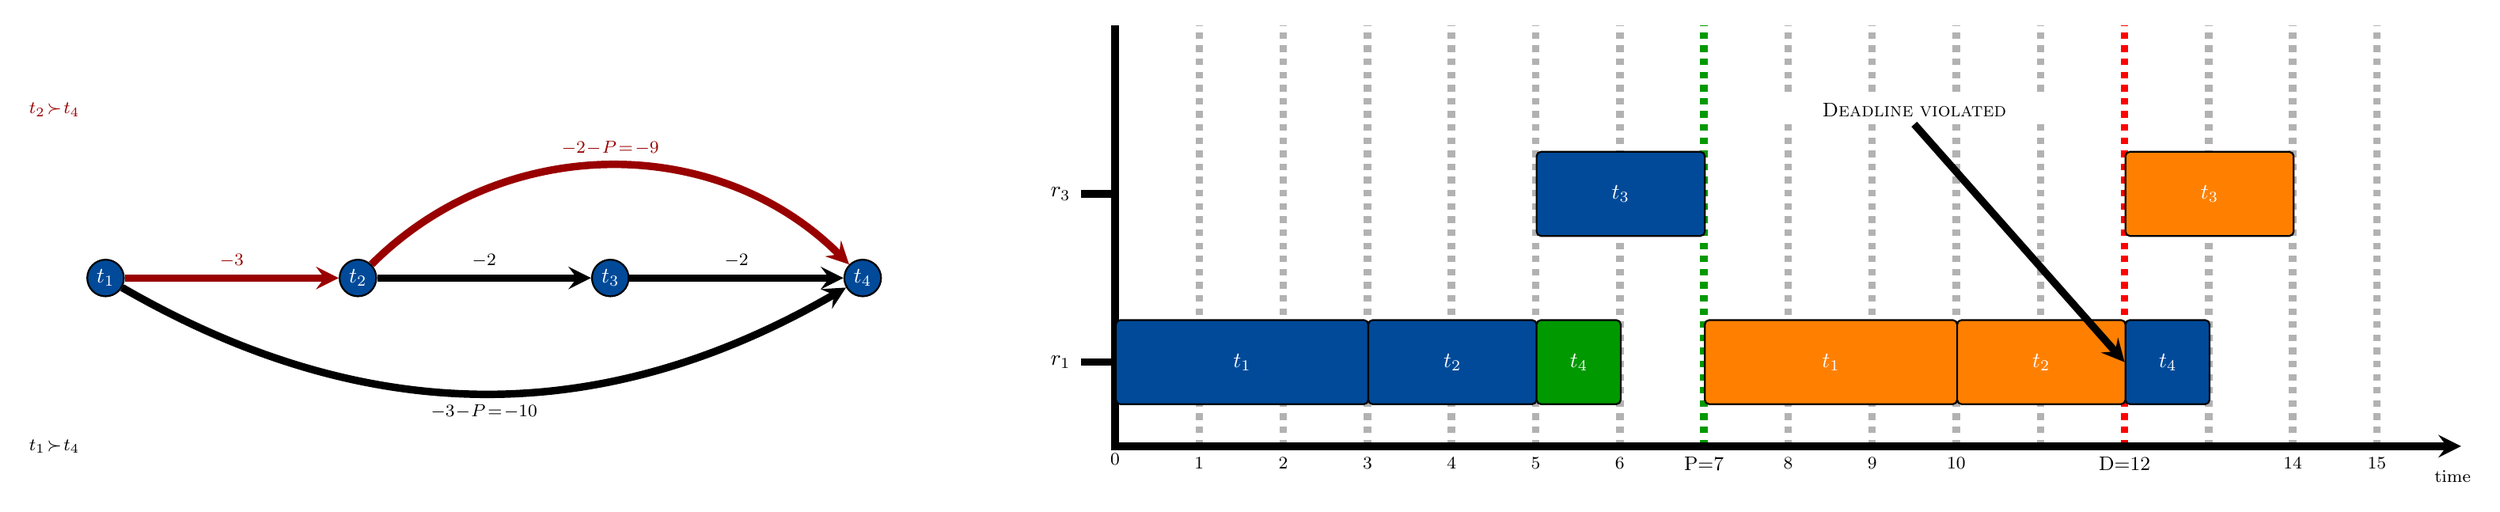
\begin{tikzpicture}[>=stealth,scale=2.7]
    \tikzstyle{axis} = [->, black, line width = 0.12cm]
    \tikzstyle{task} = [anchor=west,shape=rectangle,thick,text=white, draw=black, fill=myblue, align=center, rounded corners=2,inner sep=0, minimum height=1.35cm]
    \tikzstyle{difftask} = [shape=circle,thick,text=white,minimum height=0.5cm, draw=black, fill=myblue, align=center,inner sep=2]
    \draw[dashed, black!30] (-2.5,0) node[below, black]{\footnotesize 0};
    \foreach \i in {1,...,6}
    {
    	\draw[dashed, black!30, line width = 0.12cm] (\i*0.5-2.5,0) node[below, black]{\footnotesize\i}-- (\i*0.5-2.5,2.5);
    }
    \foreach \i in {8,...,10}
    {
    	\draw[dashed, black!30, line width=0.12cm] (\i*0.5-2.5,0) node[below, black]{\footnotesize\i}-- (\i*0.5-2.5,2.5);
    }
    	\draw[dashed, black!30, line width=0.12cm] (11*0.5-2.5,0) node[below, black]{}-- (11*0.5-2.5,2.5);
    	\draw[dashed, black!30, line width=0.12cm] (13*0.5-2.5,0) node[below, black]{}-- (13*0.5-2.5,2.5);
    \foreach \i in {14,...,15}
    {
    	\draw[dashed, black!30, line width=0.12cm] (\i*0.5-2.5,0) node[below, black]{\footnotesize\i}-- (\i*0.5-2.5,2.5);
    }
    
    \draw[black, line width = 0.12cm] (-2.5,0.5) --  (-2.7,0.5) node[left]{$r_1$};
    \draw[black, line width = 0.12cm] (-2.5,1.5) --  (-2.7,1.5) node[left]{$r_3$};
    \draw[dashed, black!40!green, line width = 0.12cm] (1,0) node[below, black]{\small P=7}-- (1,2.5);
    \draw[dashed, red, line width = 0.12cm] (3.5,0) node[below, black]{\small D=12}-- (3.5,2.5);
    \draw [axis] (-2.5,2.5) -- (-2.5,0) -- (5.5,0);
    \node[task, minimum width=4.05cm] at (-2.5,0.5) {$t_1$};
    \node[task, minimum width=2.7cm] at (-1,0.5) {$t_2$};
    \node[task, minimum width=2.7cm] at (0,1.5) {$t_3$};
    \node[task, minimum width=1.35cm,text width=1.35cm] (v5) at (3.5,0.5) {$t_4$};
    
    \node [difftask] (v1) at (-8.5,1) {$t_1$};
    \node [difftask] (v2) at (-7,1) {$t_2$};
    \node [difftask] (v3) at (-5.5,1) {$t_3$};
    \node [difftask] (v4) at (-4,1) {$t_4$};
    \draw [axis,black!40!red] (v1) edge node[above,black!40!red]{\footnotesize$-3$} (v2);
    \draw [axis] (v2) edge node[above]{\footnotesize$-2$}(v3);
    \draw [axis] (v3) edge node[above]{\footnotesize$-2$}(v4);
    \draw [axis] (v1) edge[bend right] node[below]{\footnotesize$-3-P=-10$} (v4);
    \draw [axis,black!40!red] (v2) edge[bend left=45] node[above,black!40!red]{\footnotesize$-2-P=-9$} (v4);
    
    
    \node[task, minimum width=4.05cm,fill=orange] at (1,0.5) {$t_1$};
    \node[task, minimum width=2.7cm,fill=orange] at (2.5,0.5) {$t_2$};
    \node[task, minimum width=2.7cm,fill=orange] at (3.5,1.5) {$t_3$};
    \node[task, minimum width=1.35cm,fill=black!40!green,text width=1.35cm] at (0,0.5) {$t_4$};
    
    \node[anchor=west,black!40!red] at (-9,2) {\footnotesize$t_2\succ t_4$};
    \node[anchor=west] at (-9,0) {\footnotesize$t_1\succ t_4$};
    \node[anchor=north] at (5.45,-0.1) {\footnotesize{time}};
    
    \node[fill=white,draw=none,font=\small,text width=4.5cm,align=center] (v6) at (2.25,2) {\textsc{Deadline violated}};
    \draw[axis] (v6.south) -- (v5.west);
\end{tikzpicture}

	}
	\vspace*{-3mm}
	\caption{(a) Constraint graph $G_\mathbb{C}$ based on application $A_1$ and the order $\succ$ decided by the ASP-solver. (b) The corresponding  schedule (snapshot) visualized by a Gantt chart. The variant colors represent different iterations: blue indicates the current, orange the next, and green the previous iteration.}
	\label{fig:periodicschedule1}
	\vspace*{-6mm}
\end{figure*}
\subsubsection{Check for periodic overlapping}
Even though the constraint Graph $G_\mathbb{C}$ is now consistent, jobs that are bound to the same resource might overlap with other jobs in later iterations whenever the deadline $D_{H,i}$ is greater than the hyper period $P_H$. This is checked by a dedicated propagator.
Each job that is executed later than the first period is identified as a candidate for overlapping.
%For them, the iterations they are executed in are calculated.
Now, the execution time span of all other jobs on the same resources is projected to the iterations of the candidates in question.
If the time span overlaps with the candidates time span, 
a timing constraints has to be added to serialize the execution on the same resource in that iteration.
Let $t_x \in A_i$ be the candidate and $t_y\in A_j$ be a job mapped to the same resource $r$, for which a conflict has been found.
If $t_x\succ t_y$, the constraint $\tau(t_x)-\tau(t_y)\leq -e((t_x,r))+i_r\cdot P_j$ is added to $\mathbb{C}$,
where $i_r$ is the difference between the iteration the conflict was found in and the first iteration $t_y$ is executed in.
This forces $t_x$ to be executed before $t_y$ in the iteration where an overlapping was found.
Analogously, if $t_y\succ t_x$, the constraint $\tau(t_y)-\tau(t_x)\leq -e((t_y,r))-i_r\cdot P_j$ is added to $\mathbb{C}$, forcing $t_x$ to be executed after $t_y$.
In case no overlapping has been found, $v$ is a valid partial assignment. 
If $\mathcal{B}$ and $\mathcal{R}$ are total assignments, $v$, $\mathcal{B}$, and $\mathcal{R}$ form a feasible implementation.
Otherwise, the ASP solver proceeds with binding and routing.
If overlapping was detected, we return to $1)$ with the extended set of constraints $\mathbb{C}$.


As an example for the scheduling process, we consider application $A_1$ from Figure \ref{fig:specmodel}. 
For the sake of brevity, we assume the communication between tasks to be instantaneous, i.e. the execution of a job $t_x$ is only dependent on its direct predecessor job(s). Furthermore, we presume the tasks $t_1, t_2$ and $t_4$ to be mapped to resource $r_1$ and $t_3$ to be mapped to $r_3$. 
In the first step, a constraint graph $G_\mathbb{C}$ is built upon the dependencies and execution times. %(c.f. Eq.~\eqref{const:commsame} and \eqref{const:commfirst}). 
This is represented by the black arrows in Fig.~\ref{fig:periodicschedule1}~(a). 
By calculating the shortest path to each node of $G_\mathbb{C}$, we get the initial start times for the first iteration: $\tau(t_1)=0,\ \tau(t_2)=3,\ \tau(t_3)=5,\ \tau(t_4)=7$. 
As the period $P_1$ of $A_1$ is equal to $7$, the post propagator detects periodic overlapping between task $t_1$ and $t_4$. 
As a consequence, they have to be serialized. Considering $t_1\succ t_4$, the constraint \mbox{$t_1-t_4\leq -e(t_1)-i_r\cdot P_1=t_1-t_4\leq -10$} is added with $i_r=1$ since the overlap occurs one iteration apart (red arrow). 
Now, $t_4$ overlaps with $t_2$ in the second iteration and, assuming $t_4\succ t_2$, the constraint $t_4-t_2\leq -e(t_4)+i_r\cdot P_1=t_4-t_2\leq 6$ is added, forcing $t_2$ to be executed one time step later (green arrow). 
Finally, all overlaps have been resolved and $G_\mathbb{C}$ in Fig.~\ref{fig:periodicschedule1}~(a) represents a valid schedule which is visualized by a Gantt chart in Fig.~\ref{fig:periodicschedule1}~(b). 
Note that $t_4\succ t_1$ would introduce a constraint forming a negative cycle in the constraint graph $G_\mathbb{C}$.

\subsection{Experimental Results}
Various specification instances consisting of a set of series-parallel applications as well as an architectural template implementing a regular, heterogeneous NoC have been generated randomly to test the proposed approach. All test cases were executed on a Core i7-5600U with 16~GiB RAM and a timeout of $1800\ s$. As shown in Tab.~\ref{tab:results}, our experiments indicate that ASPmT using partial assignment evaluation leverages promising results. In particular, the number of choices necessary to find a valid implementation when utilizing partial assignment checking is approximately one order of magnitude smaller compared to the evaluation of full assignments only. While the number of conflicts and average conflict length are comparable between both approaches, it shows that the search space is pruned more efficiently.

Nevertheless, the reduction of necessary choices does not correlate with the overall runtime for all test cases. As seen in Tab.~\ref{tab:results}, most of the time is spend in the background propagators when using partial assignment checking. As this is still work in progress, the performance of said propagators are subject to implementational improvements in future iterations.


%Figure~\ref{fig:periodicschedule1} shows an example of the scheduling process.
%For simplicity, we assume communication to be instantaneous but each task depends on the execution of the task before
%and constraints \eqref{const:zero} and \eqref{const:dl} are implied.
%For the example, we observe $B=\{t_1\rightarrow r_1,t_2\mapsto r_1,t_3\mapsto r_2, t_4\mapsto r_1\}$ 
%and the resulting set of constraints $C=\{t_1-t_2\leq -3,t_2-t_3\leq -2,t_3-t_4\leq -2\}$. 
%Originally, tasks $t_1$ to $t_4$ are assigned time points $0$, $3$, $5$, and $7$ respectively.
%$t_4$ is the only task to exceed the period $p=7$ and hence is the only candidate.
%We detect that $t_1$ and $t_4$ overlap in the second iteration on resource $r_1$.
%Assuming that $t_1\succ t_4$, we add the constraint $t_1-t_4\leq -e(t_1)-i_r\cdot p=t_1-t_4\leq -10$, with $e(t_1)=3$ and $i_r=1$ since the overlap occurs one iteration apart.
%The resulting constraint set is still consistent and the assignment of $t_4$ is changed to $10$.
%Now, $t_4$ overlaps with $t_2$ in the second iteration
%and, assuming $t_4\succ t_2$, we add the constraint $t_4-t_2\leq -e(t_4)+i_r\cdot p=t_4-t_2\leq 6$,
%forcing $t_4$ to be executed before $t_2$ in the next iteration.
%Figure~\ref{fig:periodicschedule1}(a) shows the resulting valid constraint graph and Figure~\ref{fig:periodicschedule1}(b) the periodic schedule.




\section{Conclusion and Future Work}
\label{sec:conclusion}
In this paper, we presented a novel ASPmT-based approach towards symbolic system synthesis that supports a more expressive system model compared to previous work. Especially, the proposed approach allows for the description of deadline-constrained periodic applications as well as heterogeneous hardware architectures.
Furthermore, the tight integration of QF--IDL into the ASP solver allows us to evaluate partial assignments in order to prune the search space more efficiently. 
First experimental results showed the general applicability of our approach. 

In the future, we aim to improve the performance of used propagators for example by using lazy variable creation or incorporating domain-specific heuristics. 
Since our ASPmT framework encompasses all relevant information,
the model is easily adaptable and features may be added comfortably.
Namely, we will extend the framework towards design space exploration including multi-objective optimization techniques.
%\blindtext
%\begin{itemize}
% \item introduce system using ASP modulo theory with following advantages:
% 	\begin{itemize}
% 		\item more expressive synthesis model
% 		\item efficient solving due to detection of invalid schedules for partial bindings,routings
% 		\item periodic scheduling without introducing new tasks
% 		\item formulation encompassing binding, routing and scheduling
% 	\end{itemize}
% \item promising results for previous synthesis model
% \item currently not scalable for periodic schedules due to many unnecessary choices, alleviated by adding variables lazily in the future
% \item scales up to NxN with Y apps with Z comms
% \item future capabilities
% 	\begin{itemize}
% 		\item multi-objective optimization
% 		\item subset of representative optimal design points
% 	\end{itemize}
% \item future techniques
% 	\begin{itemize}
% 		\item domain-specific heuristic similar to \cite{Andres2015}
% 		\item additional propagators (acyclicity)
% 	\end{itemize}
%\end{itemize}
%\begin{table}[]
%	\centering
%	\caption{My caption}
%	\label{my-label}
%	\begin{tabular}{@{}llll@{}}
%		\toprule
%		\#Resources              & \#Tasks & \#Apps & Time     \\ \midrule
%		\multirow{2}{*}{$2\times2$} & 20      & 1      & 2.08s    \\
%		& 28      & 2      & 4.85s    \\\midrule
%		\multirow{4}{*}{$3\times3$} & 27      & 1      & 8.24s    \\
%		& 45      & 5      & 13.99s   \\
%		& 45      & 2      & 121.28s  \\
%		& 45      & 1      & TO       \\\midrule
%		\multirow{5}{*}{$4\times4$} & 48      & 3      & 191.871s \\
%		& 48      & 1      & 280.86s  \\
%		& 80      & 6      & 543s     \\
%		& 80      & 5      & 577.63s  \\
%		& 80      & 1      & TO       \\\midrule
%		$5\times5$                  & 75      & 5      & TO       \\ \bottomrule
%	\end{tabular}
%\end{table}


\section*{Acknowledgment}
This work was funded by the German Science Foundation (DFG) under grants HA 4463\slash4-1 and SCHA 550/11-1.
%Blinded for review.
\footnotesize
\bibliographystyle{unsrt}
\bibliography{library}%,lit,akku,procs}





% trigger a \newpage just before the given reference
% number - used to balance the columns on the last page
% adjust value as needed - may need to be readjusted if
% the document is modified later
%\IEEEtriggeratref{8}
% The "triggered" command can be changed if desired:
%\IEEEtriggercmd{\enlargethispage{-5in}}

% references section

% can use a bibliography generated by BibTeX as a .bbl file
% BibTeX documentation can be easily obtained at:
% http://mirror.ctan.org/biblio/bibtex/contrib/doc/
% The IEEEtran BibTeX style support page is at:
% http://www.michaelshell.org/tex/ieeetran/bibtex/
%\bibliographystyle{IEEEtran}
% argument is your BibTeX string definitions and bibliography database(s)
%\bibliography{IEEEabrv,../bib/paper}
%
% <OR> manually copy in the resultant .bbl file
% set second argument of \begin to the number of references
% (used to reserve space for the reference number labels box)
%\begin{thebibliography}{1}
%
%\bibitem{IEEEhowto:kopka}
%H.~Kopka and P.~W. Daly, \emph{A Guide to \LaTeX}, 3rd~ed.\hskip 1em plus
%  0.5em minus 0.4em\relax Harlow, England: Addison-Wesley, 1999.
%
%\end{thebibliography}




% that's all folks
\end{document}
